% Qual o problema? porque é bom ter geração procedural terrenos
% \section{Introdução}

\begin{frame}{Contextualização}
  \begin{itemize}
        \item Criar conteúdo para jogos manualmente exige muito tempo de trabalho
        \item Conteúdo criado manualmente exige persistência do próprio conteúdo
    \end{itemize}
\end{frame}

\begin{frame}{Contextualização}
    \begin{figure}
		\centering
        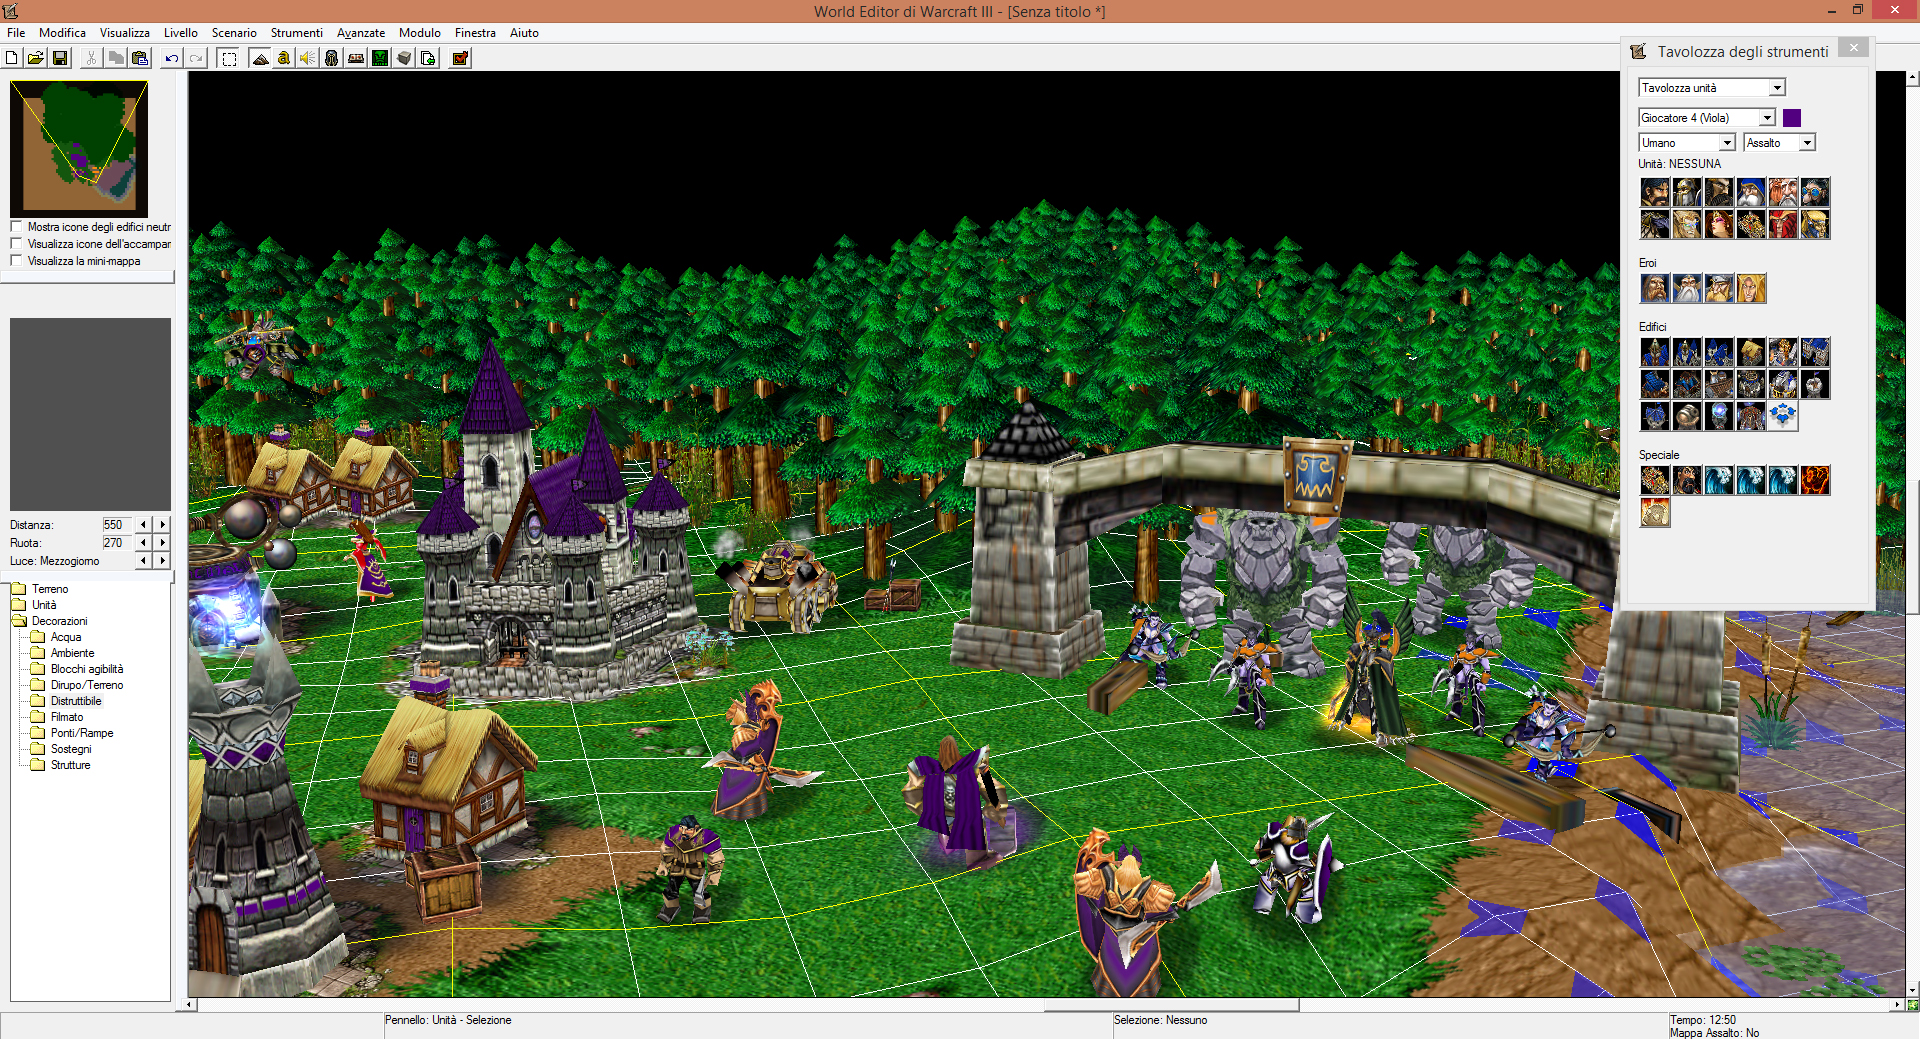
\includegraphics[width=.8\textwidth]{img/intro/World_Editor_di_Warcraft_III.jpg}
        \caption{Editor de mapas do \alert{Warcraft III}}
    \end{figure}
    \url{it.wikipedia.org/wiki/World_Editor_di_Warcraft_III}
\end{frame}

\begin{frame}{Contextualização}
    \begin{itemize}
        \item Conteúdo criado proceduralmente exige persistência do método(Algoritmo)
        \item Quanto maior o mundo virtual, tecnicamente mais tempo os jogadores irão explorar \cite{bevilacqua2009ferramenta}
    \end{itemize}
\end{frame}


\begin{frame}{Contextualização}
    \begin{figure}
		\centering
        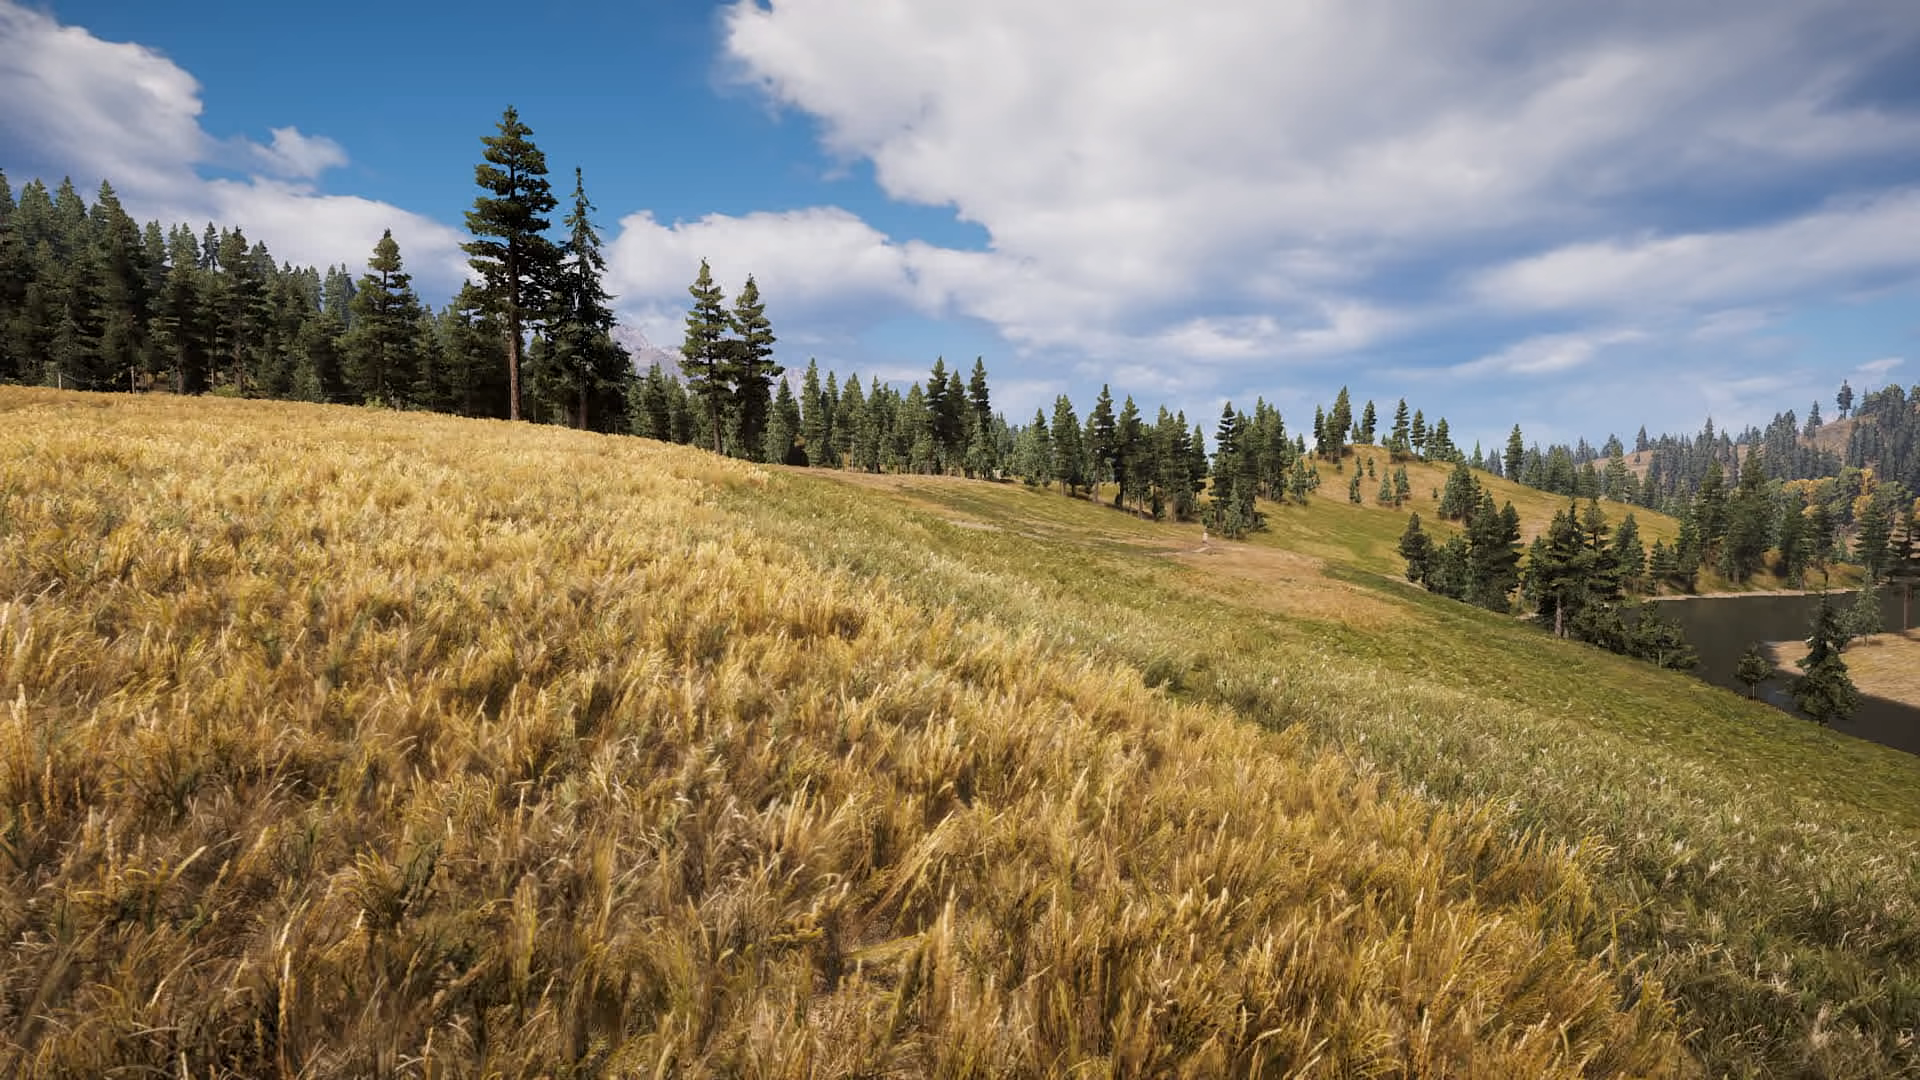
\includegraphics[width=.8\textwidth]{img/intro/fc5terrain.png}
        \caption{Mapa de \alert{Far Cry 5}, \cite{Carrier2018farcry5}}
    \end{figure}
\end{frame}

\begin{frame}{Contextualização}
    \begin{figure}
		\centering
        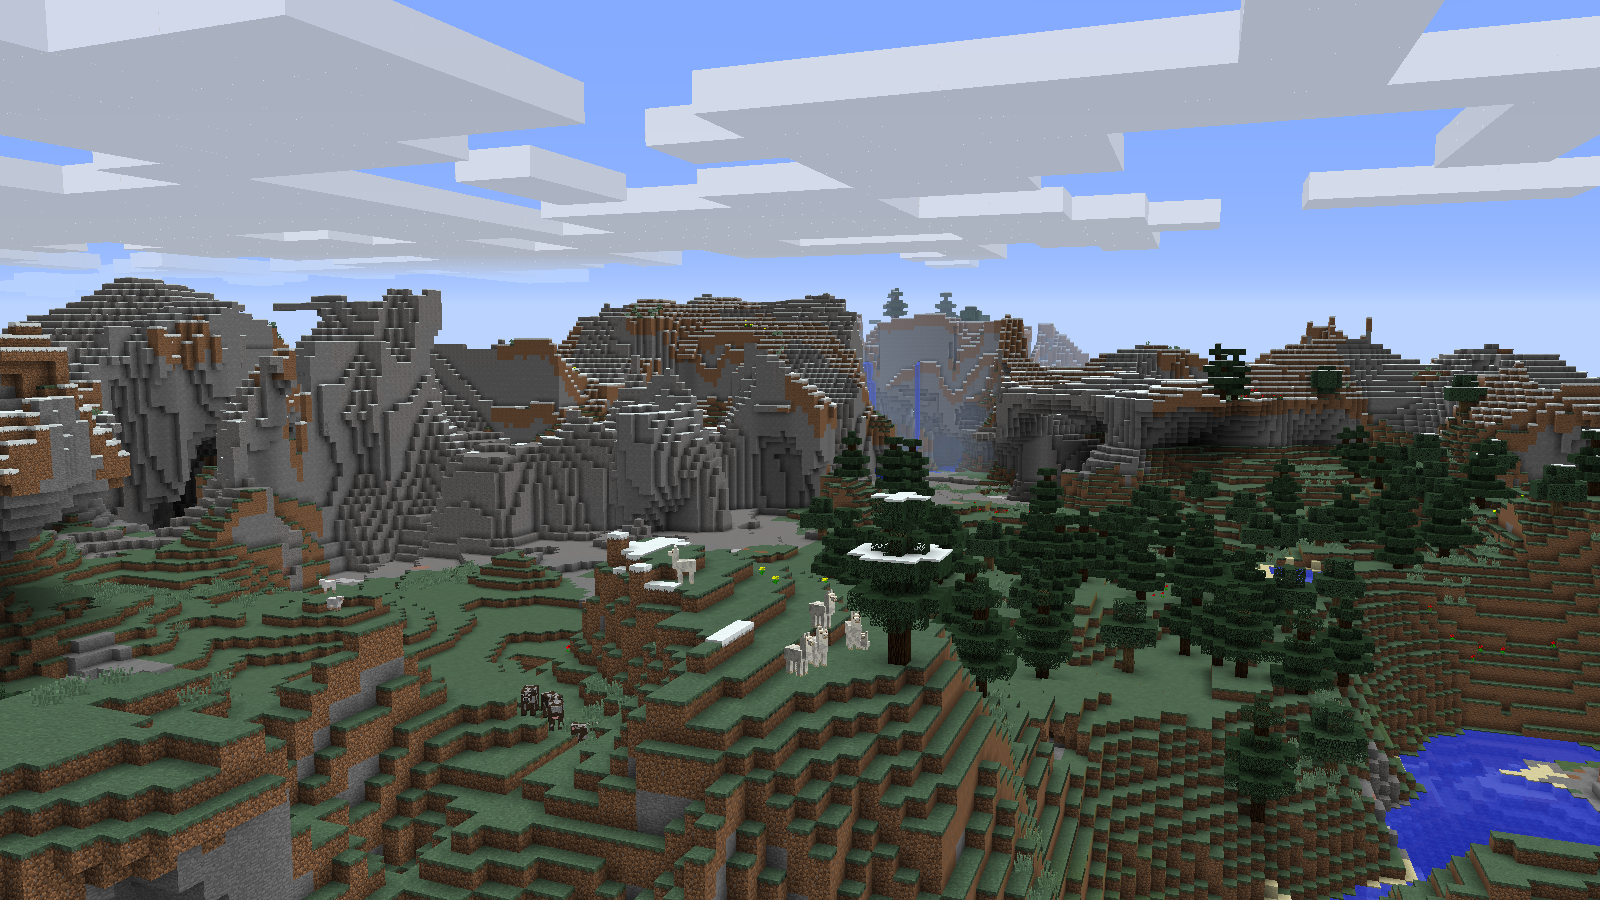
\includegraphics[width=.8\textwidth]{img/intro/mineExtremeHills.png}
        \caption{Mundo de \alert{Minecraft}}
    \end{figure}  
\end{frame}

\begin{frame}{Objetivo}
    \begin{itemize}
        \item Mostrar um método capaz de gerar um terreno para jogos
        \item Terrenos com relevos \alert{naturais}
    \end{itemize}
\end{frame}